Vision is the ability to make inferences about the natural world from the
patterns of light captured by the eyes of living organism or cameras in
machines. A digital image is a discrete two dimensional array of intensity
values referred to as pixels. Though each pixel corresponds to a potentially
independent light intensity measurement, these intesities exhibit strong
spatial correlations in natural images \cite{simoncelli2001}.  However, this
structure is not explicitly captured by the camera sensor; each pixel is stored
as a separate light intensity measurement in memory. Therefore it is natural to
think of raw images as points in high dimensional space in which each pixel
corresponds to an independant variable. Fundamentally, the structure in images
is due to the structure of our world; though no two objects are exactly alike,
many structures and textures are repeated throughout the world allowing us to
categorize and identitfy objects by referencing our memory.  Because of this
structure, or dependency among the pixels, the number of possible
\emph{natural} images is far smaller than the number of possible images.  This
observation has a geometric interpretation: the \emph{intrinsic} dimension of
natural images is much lower than the ambient dimension, thus natural images
are concentrated around low-dimensional ``manifolds''
\cite{bengio2013,tenenbaum2000,roweis2000}. Similarly, videos can be imagined
as one dimensional trajectories on this manifold parametrized by time
\cite{goroshin2015}. In contrast to natural images, random images contain no
structure by contruction. Thus a collection of random images fills the ambient
space, rather then concentrating on low dimensional manifolds.  Figure
\ref{fig:structure} is an illustrative visualization of the distribution of
random images (left) and natural images (right). 

The role of visual features is to transform the raw input image to a
representation that facilitates inferences about the natural world by modeling
commonly occurring dependencies between input pixels. This can be restated from
the manifold perspective: visual features model the natural data manifold.  The
manifold theory of natural data allows for a more geometrically intuitive
interpretation of problems in computer vision. Many existing feature learning
algorithms will be presented from the manifold theory perspective of natural
data in Chapter \ref{chapter:related_work}. 

\begin{figure} 
\centering
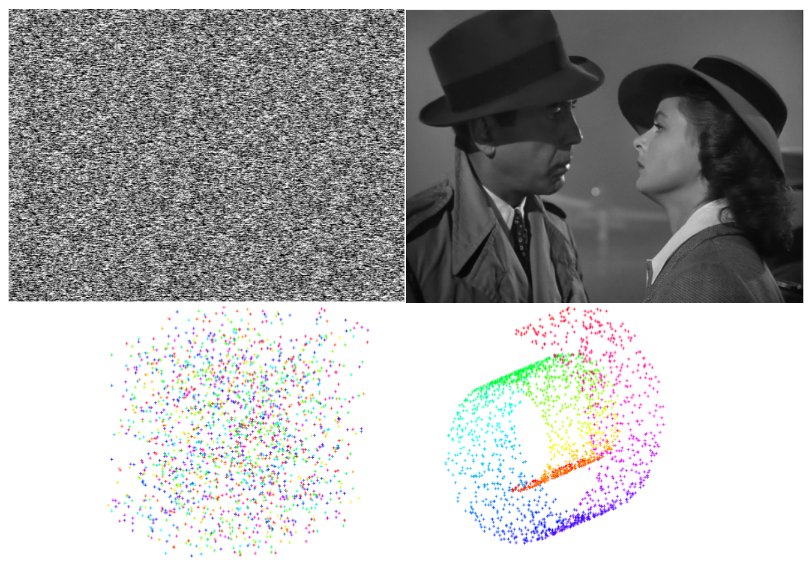
\includegraphics[scale=0.3]{./figures/introduction/structure.png} 
\caption{Top left: random image, Top right: natural image, Bottom left: visualization of
unstructured data, Bottom right: visualization of data with intrinsic
structure} 
\label{fig:structure} 
\end{figure}  

Historically, approaches for constructing visual features in computer vision
have been broadly divided into two categories: ``hand-crafted'' features are
designed by a human expert, whereas ``learned'' features use techniques from
machine learning to learn the features automatically from the problem related
data itself. Examples of hand crafted features (also called ``descriptors'')
include the Scale Invariant Feature Transform (SIFT) \cite{SIFT}, Histogram of
Gradients (HoG) \cite{HoG}, and ``gist'' \cite{gist} features. Though these
hand crafted features paved the way for many breakthroughs in computer vision,
recent breakthroughs have largely been attributed to feature learning with deep
convolutional networks (ConvNets) \cite{fukushima1980, LeCun1998, ImageNet}.
Remarkably, these hand-crafted features bear striking similarity to shallow
ConvNets. The main differences between ConvNets and these features are that:
(i) ConvNet features are optimized or ``learned'' for specific problems, and
(ii) they are arranged and learned in a hierarchical fashion. Traditional
ConvNet layers are composed of trainable convolutional filter banks,
interspersed with point-wise nonlinearities and sub-sampling (or ``pooling'')
layers.  A now famous ConvNet architecture, dubbed LeNet5 \cite{LeCun1998} is
shown in Figure \ref{fig:LeNet5}.       

\begin{figure} 
\centering
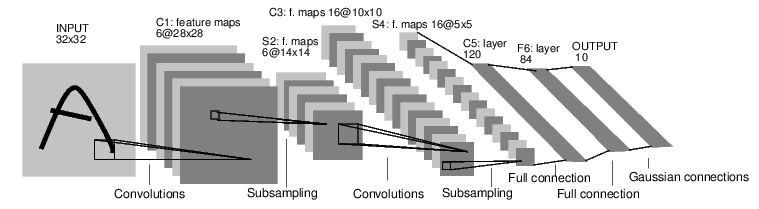
\includegraphics[scale=0.5]{./figures/introduction/lenet5.png} 
\caption{The LeNet5 network was trained to recognize hand written characters in order to 
automatically process bank checks} 
\label{fig:LeNet5} 
\end{figure}  

Interestingly, the hierarchical representations of ConvNets were inspired by
studies of natural visual systems. A long standing belief in neuroscience is
that the visual cortex also has a hierarchical organization
\cite{hubel1968,felleman1991}. Simply put, there is a sequence of processing
steps which eventually results in our visual perception of the world. Recent
work has revealed strong empirical similarities between the artificial feature
hierarchies of ConvNets and natural visual hierarchies of the animal visual
system \cite{yamins2014}. Though the hierarchical representations learned by
ConvNets are not completely understood, it is clear that the sequence of
operations corresponding to each layer transforms the data in a way that makes
the task easier to solve for the final layer, often a linear operator.    

Deep hierarchical features have the capacity to represent highly complex
structures that embody abstract invariances. Hand crafting effective feature
hierarchies that embody these properties is an intratractable task. There is
strong biological and psychological evidence of learning in the visual
coretices of humans and animals \cite{foldiak1991,sinha2013}. In a project lead by    
Pawan Sinha that restored vision to young adults affected by congenital cataracts, 
the subjects took several weeks to learn how to see \cite{sinha2013}. There is even
evidence to support the existiance of learning principle that is agnostic to
sensory modality \cite{sharma2000}.   

Recent findings suggest that the early stages of the hierarchy learned by ConvNets 
on specific \emph{supervised learning} tasks such as classification, can be transfered 
to other tasks, such as segmentation \cite{yosinski2014}. This finding suggests 
that these representations are not task specific but are generically useful. 
The goal of this thesis is to explore \emph{unsupervised learning} principles that lead
to generically useful hierarchical representations.    

\section{Thesis Outline and Summary of Contributions} 

The thesis is organized as follows. In Chapter \ref{chapter:related_work}
reviews prior work on feature learning with emphasis on auto-encoders and
sparse feature learning.  Chapter \ref{chapter:SATAE} introduces the Saturating
Auto-Encoder, a class of regularized auto-encoders whose regularizers play an
analogous role to the partition function of probabilistic models. The new
regularizer offers a unified interpretation of other popular
regularizered auto-encoders such as the Sparse Auto-Encoder and Contractive
Auto-Encoder \cite{SAE,CAE}. Because learning sparse inference will play an
important role in later chapters, Chapter \cite{LISTA} evaluates various
network architectures for learning sparse inference in pre-trained and learned
dictionaries. Chapters \ref{chapter:slow} and \ref{chapter:linear} propose 
new methods for learning hierarchical features from temporally coherent data (video).        
Chapters \ref{chapter:slow} introduces an architecture and loss to learn spatio-temporally
coherent metrics that parallels Slow Feature Analysis \cite{SFA}. We show that 
the learned metrics exhibit \emph{semantic} coherence by evaluating them on a class-based recall 
task. In Chapter \ref{chapter:linear} we propose a new architecture and loss for learning 
features that \emph{linearize} temporal transformations in natural video. We also 
introduce the ``phase-pooling'',an operator specifically designed for the task of linearization. 
Finally, Chapter \ref{chapter:conclusion} concludes the thesis and points future research 
directions. 






